\section{PROFINET-Verbindung} \label{sec:ergebnisse}

\subsection{Verbindung herstellen} \label{sec: Verbindung herstellen}
Die PROFINET-Verbindung beider Geräte und deren Module wird über die \textbf{Netzsicht} vorgenommen. Dabei ist auf die richtigen Anschlüssen zu achten (s. \autoref{sec: IP-Adresse_PROFINET-Gerätename_S7-1500} und \autoref{sec: IP-Adresse_PROFINET-Gerätename_ET_200SP}).

\begin{figure}[H]
   \centering
   \fbox{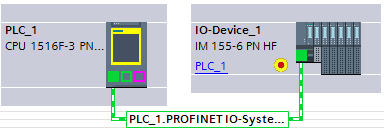
\includegraphics[width=0.8\textwidth]{Bilder/5. PROFINET-Verbindung/5.1 Verbindung herstellen/(5.1.1) PROFINET-Verbindung ziehen.png}}
   \caption[PROFINET-Verbindung herstellen]{PROFINET-Verbindung herstellen}
   \label{fig:Bild5.1}
\end{figure}

\subsection{Fehlersicherheit aktivieren}
Zusätzlich zur PROFINET-Verbindung in der Netzsicht ist in den Einstellungen der S7-1500 (über \textbf{Gerätesicht}) die Fehlersicherheit (\textbf{F-Fähigkeit}) zu aktivieren.\\
Pfad: Fehlersicherheit > F-Aktivierung

\begin{figure}[H]
   \centering
   \fbox{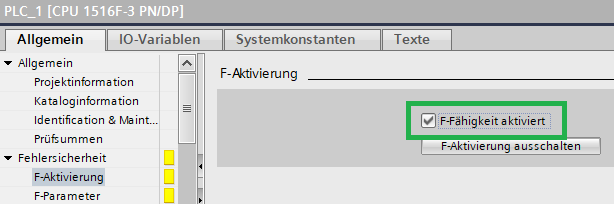
\includegraphics[width=0.8\textwidth]{Bilder/5. PROFINET-Verbindung/5.2 Fehlersicherheit aktivieren/(5.2.1) Fehlersicherheit aktivieren.png}}
   \caption[Fehlersicherheit aktivieren]{Fehlersicherheit aktivieren}
   \label{fig:Bild5.2}
\end{figure}

\subsection{Überprüfung des internen PROFINET-Gerätenamens der ET 200SP}
Möglicherweise stimmt der intern festgelegte Gerätename nicht mit dem nach \autoref{sec: IP-Adresse_PROFINET-Gerätename_ET_200SP} vergebenen überein. Um dies zu kontrollieren, kann über einen Rechtsklick auf die gesetzte PROFINET-Verbindung in der Netzsicht (s. \autoref{sec: Verbindung herstellen}) der Gerätename der ET 200SP ausgelesen und abgeglichen werden (\textbf{Rechtsklick > Gerätename zuweisen})(\autoref{fig:Bild5.3}).  Stimmen die Gerätenamen nicht überein, muss der Name entsprechend geändert werden (s. \autoref{sec: IP-Adresse_PROFINET-Gerätename_ET_200SP}).

\begin{figure}[H]
   \centering
   \fbox{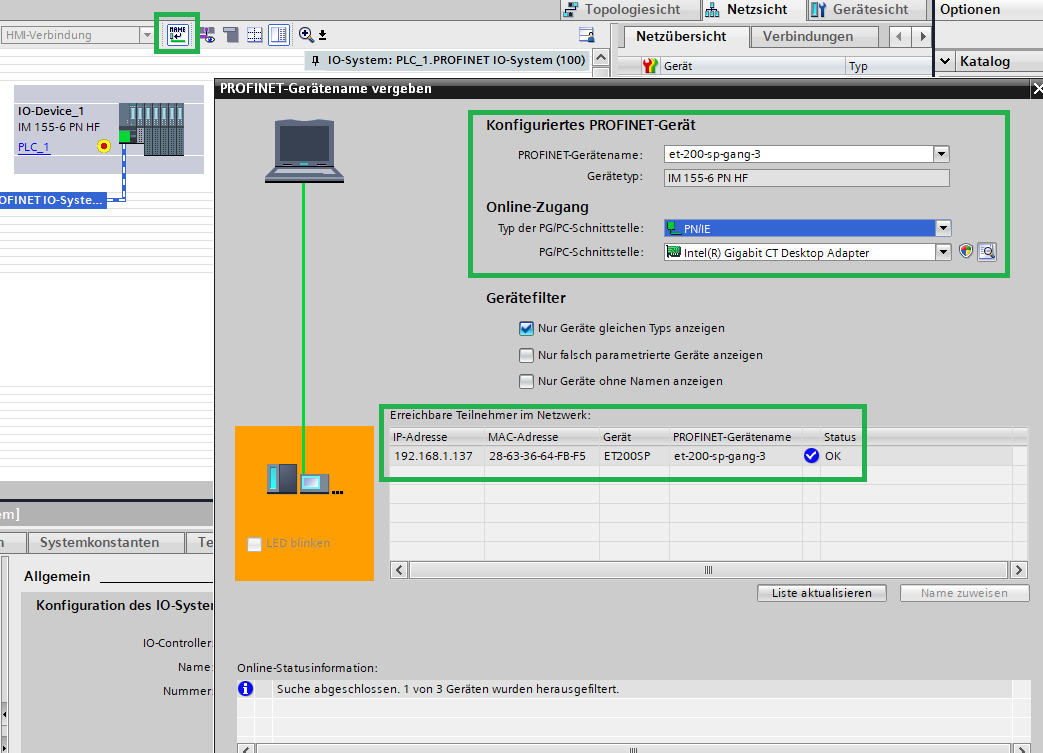
\includegraphics[width=0.8\textwidth]{Bilder/5. PROFINET-Verbindung/5.3 Überprüfung des internen PROFINET-Gerätenamens der ET 200SP/(5.3.1) Ueberpruefung der richtigen Namen.png}}
   \caption[Überprüfung des internen Gerätenamens der ET 200SP]{Überprüfung des internen Gerätenamens der ET 200SP}
   \label{fig:Bild5.3}
\end{figure}

\subsection{Überprüfung der IP-Adressen der Geräte}
Eine weitere Überprüfung für die korrekte Verbindung ist in der Netzsicht über den Button \glqq\textbf{Adressen anzeigen}\grqq\:möglich. Hierbei werden die IP-Adressen der Geräte angezeigt. Diese können mit der \autoref{fig:Bild1.3} abgeglichen werden. Sofern keine Verbindung hergestellt wurde, wird eine Fehlermeldung ausgegeben.

\begin{figure}[H]
   \centering
   \fbox{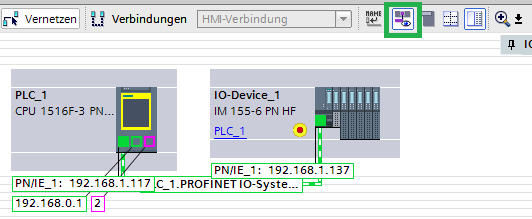
\includegraphics[width=0.8\textwidth]{Bilder/5. PROFINET-Verbindung/5.4 Überprüfung der IP-Adressen der Geräte/(5.4.1) Ueberpruefung der richtigen Adressen.png}}
   \caption[Überprüfung der IP-Adressen der Geräte]{Überprüfung der IP-Adressen der Geräte}
   \label{fig:Bild5.4}
\end{figure}